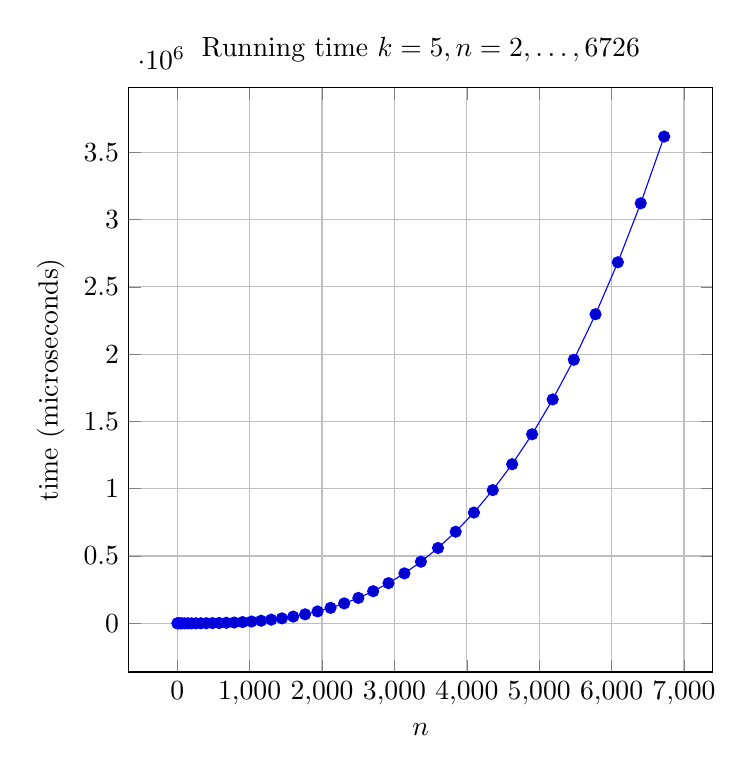
\begin{tikzpicture}
\begin{axis}[
		%xmode=log,
title={Running time $k=5,n=2,\dots,6726$},
height=9cm,
width=9cm,
grid=major,
xlabel = $n$,
ylabel = time (microseconds),
]
\addplot coordinates {
	(2,0)
	(6,0)
	(18,0)
	(38,1)
	(66,9)
	(102,24)
	(146,50)
	(198,112)
	(258,235)
	(326,466)
	(402,848)
	(486,1481)
	(578,2462)
	(678,3939)
	(786,6083)
	(902,9271)
	(1026,13357)
	(1158,19278)
	(1298,27520)
	(1446,37018)
	(1602,50129)
	(1766,66930)
	(1938,88378)
	(2118,114971)
	(2306,148055)
	(2502,188859)
	(2706,238534)
	(2918,298675)
	(3138,371052)
	(3366,457771)
	(3602,559747)
	(3846,680632)
	(4098,822848)
	(4358,989762)
	(4626,1182116)
	(4902,1404667)
	(5186,1663503)
	(5478,1958169)
	(5778,2296425)
	(6086,2682430)
	(6402,3120744)
	(6726,3616376)
};
\end{axis}
\end{tikzpicture}
